\section{软件变更分析系统设计}\label{system-design}

AOSP 是一个庞大的系统。截至 2021 年 10 月 1 日,AOSP 项目下共有 2192 个仓库。在 Android-12.0.0\_r1 版本下,一共存在 55094 个模块。AOSP 中使用的通用编程语言种类丰富,并且 AOSP 中不同种类语言实现的项目间的直接调用关系较少(如 platform/external/qemu 与 platform/frameworks/uiautomator 之间)。因此对整个 AOSP 进行代码分析不仅会带来较大的困难,同时也不具备实际意义。

本文所设计的软件变更分析系统焦于 AOSP 中 platform/frameworks 下的众多仓库与模块。platform/frameworks 中包含 Android 应用开发的核心 Java API 框架、Android 运行时以及对各种硬件的抽象封装,是 AOSP 中最为重要的开源部分之一。本系统将使用 git 版本控制系统中的数据结构获取变更,从 AOSP 构建系统 GNU Make 与 soong 的整体架构、Blueprint 组件对 bp 文件的解析、AOSP 底层构建系统 Ninja 的模块间分析能力切入,利用 AOSP 构建完成的产物进行模块内分析。本节将列出本次毕业设计过程中设计与开发的解决方案,并提出实现软件变更分析系统的解决方案。

\subsection{数据预处理}

\subsubsection{数据爬取:repo\_crawler}

由 AOSP 目录结构可知,AOSP 中仓库分布并无规则。分析单目录下仓库列表的方法有两类,一类是基于 .git 目录进行试探性测试的离线方法,一类是基于 AOSP 源码站的在线方法。该系统利用 Python 的 requests 和 bs4 获取 platform/frameworks 下所有仓库名称,该模块流程设计如图\ref{fig:archi-repo-crawler}所示。

\begin{figure}[htb]
    \centering
    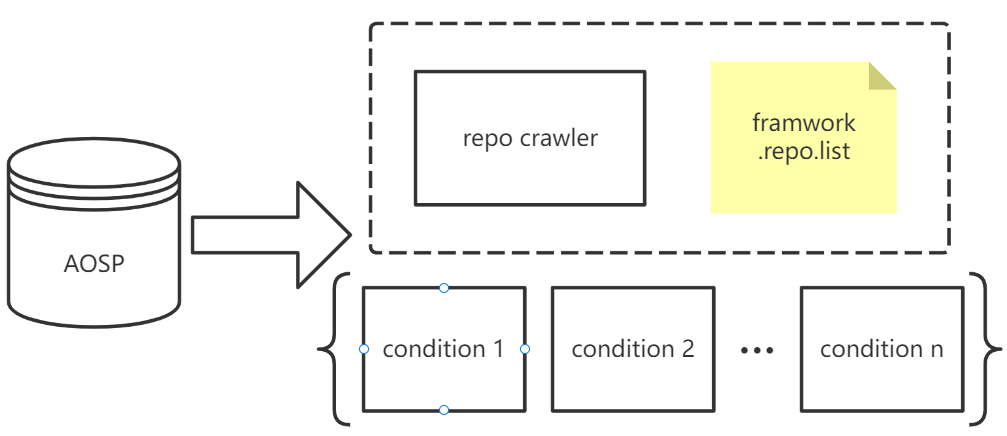
\includegraphics[width=.9\textwidth]{figures/archi-repo-crawler.png}
    \caption{repo\_crawler 设计图}
    \label{fig:archi-repo-crawler}
\end{figure}

\subsubsection{Android.bp 文件收集:bp\_collector}

soong 构建系统在运行之初会调用 Blueprint 模块。Blueprint 模块的主要执行过程大致可被分为三步:收集 Android.bp 文件,将 Android.bp 文件中的 Blueprint 语法转化为 ninja 语法,输出到 ninja manifest 文件中。soong 在运行时会输出一份从各个路径中寻找存在 Android.bp 的目录,并将该目录输出在 out/.module\_paths 下的 Android.bp.list 中。因此可以有效利用该文件收集散布于整个 AOSP 中的,且在构建过程中被使用到的 Android.bp 文件。该部分设计逻辑如图\ref{fig:archi-bp-collector}所示。

\begin{figure}[htb]
    \centering
    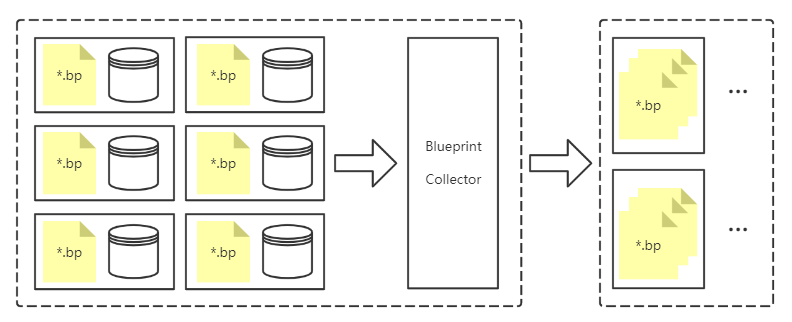
\includegraphics[width=.9\textwidth]{figures/archi-bp-collector.png}
    \caption{bp\_collector 示意图}
    \label{fig:archi-bp-collector}
\end{figure}

\subsubsection{仓库-模块关系:pkg\_repo\_tool}

根据第二步的结果,将收集到的所有 bp 文件放在一个路径下。利用 Blueprint 中的 parser 模块解析收集到的 bp 文件,使用 Go 语言编写应用程序,要求输入第一步中得到的仓库名,输出具体内部项目 / 模块 / 仓库三者之间的联系到一个 json 文件当中。该部分的架构图如图\ref{fig:archi-pkg-repo-tool}所示。

\begin{figure}[htb]
    \centering
    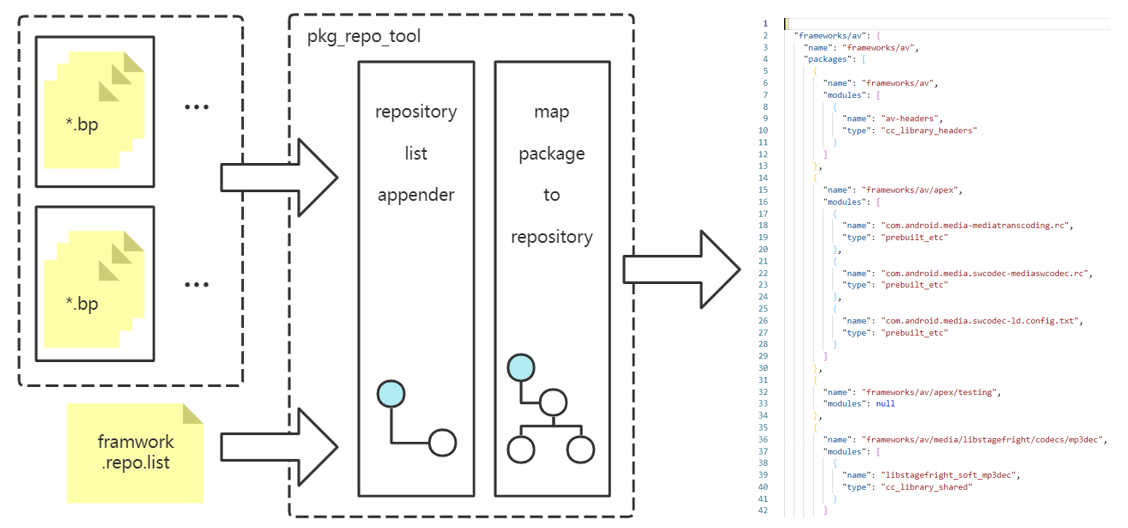
\includegraphics[width=.9\textwidth]{figures/archi-pkg-repo-tool.png}
    \caption{pkg\_repo\_tool 示意图}
    \label{fig:archi-pkg-repo-tool}
\end{figure}

\subsection{软件变更获取:diff\_extractor}

通过给定的仓库与两个版本的 commit id,可以利用 git 中的数据结构,获得两版本间存在差异的文件名。与此同时,本系统选用 GumTree 作为抽象语法树节点级别的变更获取工具,并使用算法\ref{alg:get-method-name},从 GumTree 给出的变更节点向上回溯至方法定义节点与类定义节点,进而获取两版本间存在差异的方法名与类名。该模块架构如图\ref{fig:archi-diff-extractor}所示。

\begin{figure}[htb]
    \centering
    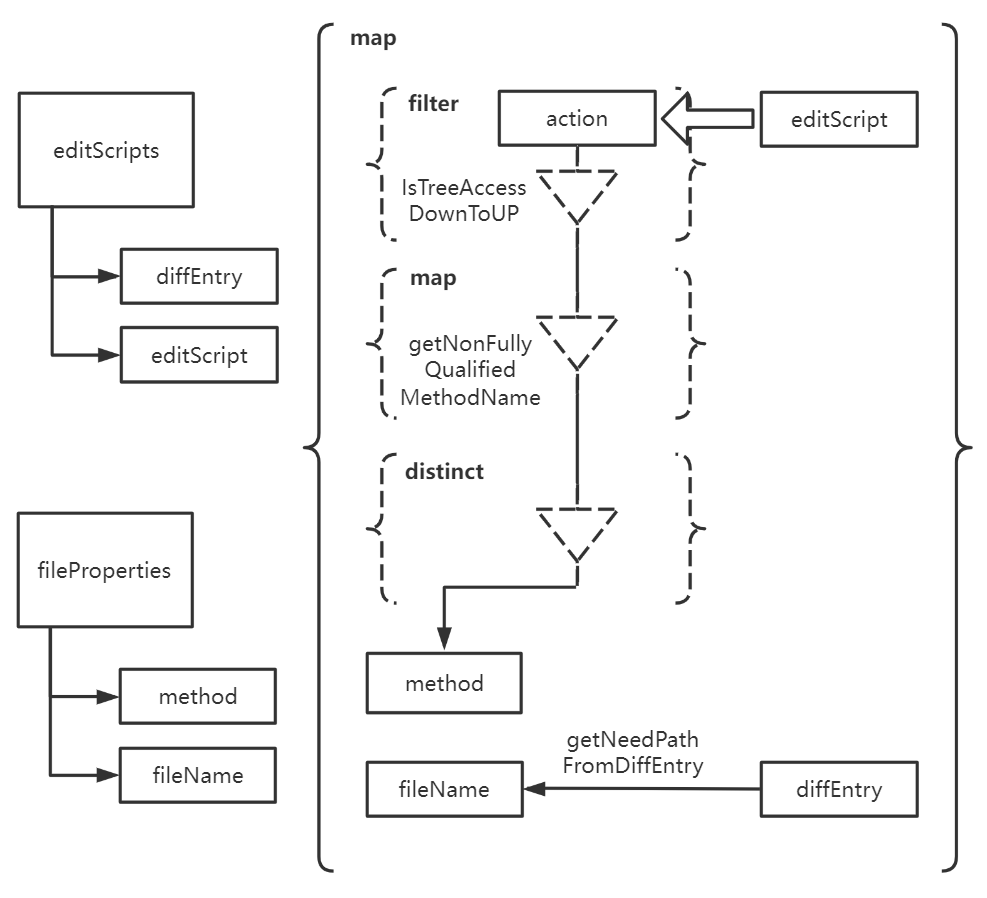
\includegraphics[width=.9\textwidth]{figures/diff-extractor-main.png}
    \caption{diff\_extractor 主函数部分实现}
    \label{fig:diff-extractor-main}
\end{figure}

对于 diff\_extractor 的具体实现而言,在选用的开源工具上,本系统使用了 eclipse.jgit 解析 git 仓库中的数据结构,并使用 GumTree 获得基于抽象语法树的细粒度软件变更。jgit 可以根据输入的信息,获得诸如变更文件名、具体变更文本以及变更前后的源代码等。该项目将变更前后的源代码传入 GumTree,再根据获得的输出基于抽象语法树节点标签判断,最终得到 json 格式的输出结果;在编程范式上,本系统使用了函数式编程与面向对象式编程相结合的编程范式,这一特点着重体现在主函数上,主函数逻辑如图\ref{fig:diff-extractor-main}所示。

\begin{figure}[htb]
    \centering
    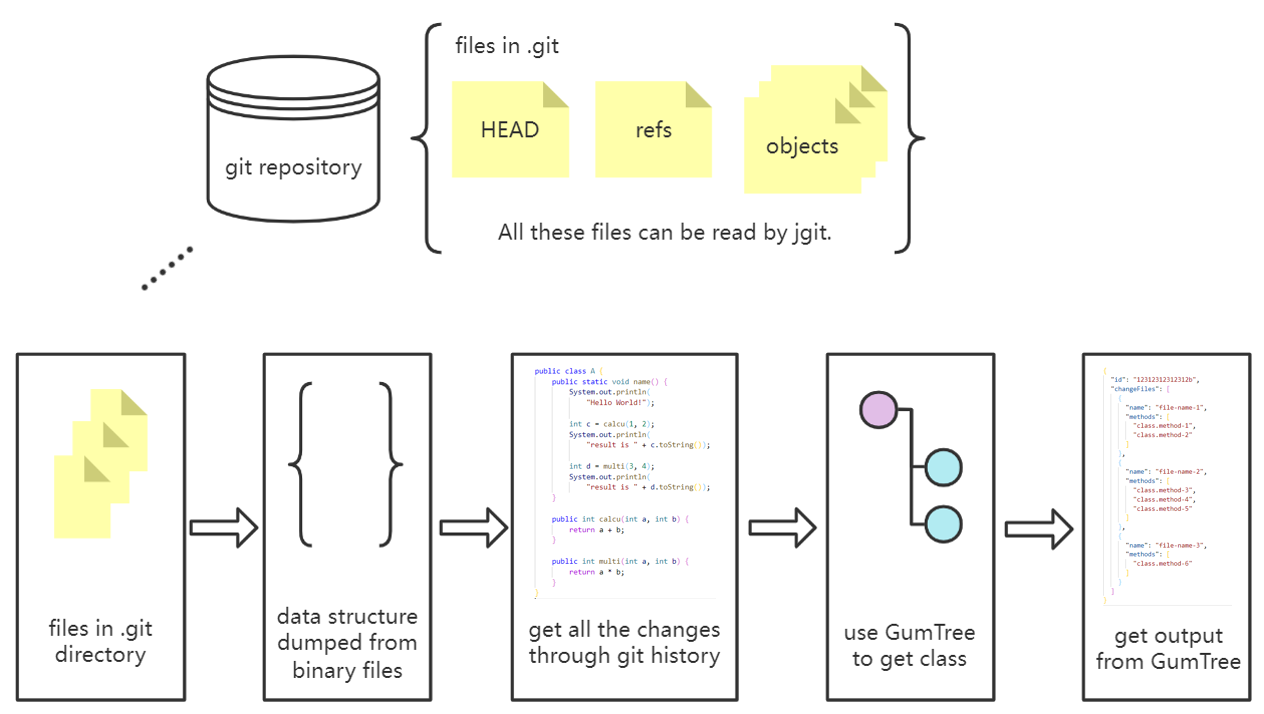
\includegraphics[width=.9\textwidth]{figures/archi-diff-extractor.png}
    \caption{diff\_extractor 示意图}
    \label{fig:archi-diff-extractor}
\end{figure}

\subsection{模块间分析功能}

\subsubsection{精简完全构建过程描述文件:manifest\_refinement}

在编译 AOSP 时,soong 构建系统中的 Blueprint 模块被自动调用生成 build.ninja 文件。然而,即便 ninja 语法相较于 Makefile 而言更为简单,用于描述 AOSP 完全构建过程的纯文本文件 build.ninja 仍需要占用 3 GB 左右的磁盘空间。对 ninja 文件进行分析依旧需要较大的资源。本系统为解决该问题,根据 Android.bp 文件所在路径使用文本匹配方法,剔除不在本系统考虑范畴之内(platform/frameworks)的构建过程。manifest 文件处理结果如图\ref{fig:archi-manifest-refinement}所示。

\begin{figure}[htb]
    \centering
    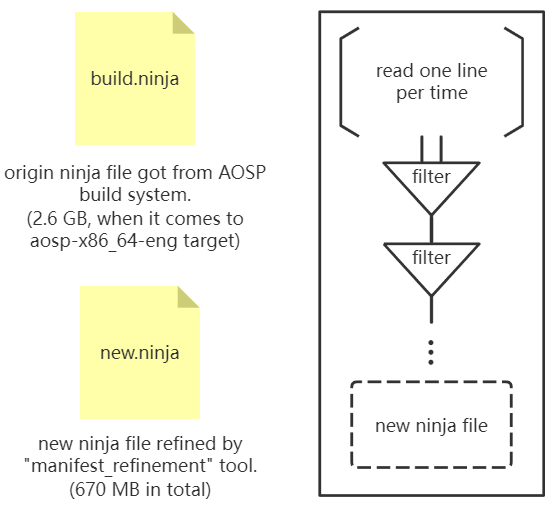
\includegraphics[width=.5\textwidth]{figures/archi-manifest-refinement.png}
    \caption{manifest\_refinement 示意图}
    \label{fig:archi-manifest-refinement}
\end{figure}

\subsubsection{求解扩展有向图中多源可达问题:ninja\_hacked}

Ninja 中使用 Node 抽象真实存在的文件,使用 Edge 抽象单一构建过程 “build”,进而利用 Node 与 Edge 数据结构构成有向无环图。在多源可达问题求解中,首先需要确定所有的存在变更的源文件。在 AOSP 的构建过程中,如果一个文件并非由 Ninja 构建系统中的构建过程给出,则说明该文件是源文件。也就是说,在 Ninja 所维护的有向无环图中,若一个 Node 仅有 in\_edge,而其 out\_edge 不存在或 out\_edge 并没有连接其余输出,则说明该 Node 对应的文件属于源文件。根据 AOSP 中 Ninja 的工作流程,存在变更的文件必定属于源文件。ninja\_hacked 项目的流程图如图\ref{fig:archi-ninja-hacked}所示。

对于图\ref{fig:archi-ninja-hacked}中的算法部分,其使用广度有限搜索(BFS)得到了图\ref{fig:ninja-hacked-bfs}中 “涂色节点”,即 “所有受给定变更文件影响的文件”——图\ref{fig:ninja-hacked-bfs}中给出了表示了最朴素的三种完全构建过程中单源可达问题场景:

\begin{enumerate}
    \item 与变更节点直接连接的构建过程只有该节点对应的源文件本身,且该节点只连接了一个构建过程;
    \item 与变更节点直接连接的构建过程有多个源文件,但该节点只连接了一个构建过程;
    \item 与变更节点直接连接的构建过程有多个源文件,且该节点连接了多个构建过程。(连接多个构建过程,但每个构建过程连接的源文件只有变更节点的情况与该栏目类似)
\end{enumerate}

(注:图中的蓝色节点表示存在变更的节点,黄色节点表示受到直接影响的节点,紫色节点表示可能因 “变更节点对应的文件中的开放 API 变更” 而受到间接影响的节点。)

ninja\_hacked 会利用 Ninja 中的定义的数据结构,基于给定的变更源文件并以此为起点,按照其连接的构建过程向上遍历,获得所有受到影响的节点。

为便于后续分析,ninja\_hacked 还需要给出文件在完全构建过程中所有受影响节点到变更节点的距离。使用算法\ref{alg:total-build-topology-sort}中描述的 “基于完全构建过程的拓扑排序算法” 思想,可以将 “当前节点连接的所有构建过程中的所有输入节点的距离最大值 + 1” 作为当前节点距离,从而解决图\ref{fig:ninja-hacked-topology-sort}中距离确定问题。

\begin{figure}[htb]
    \centering
    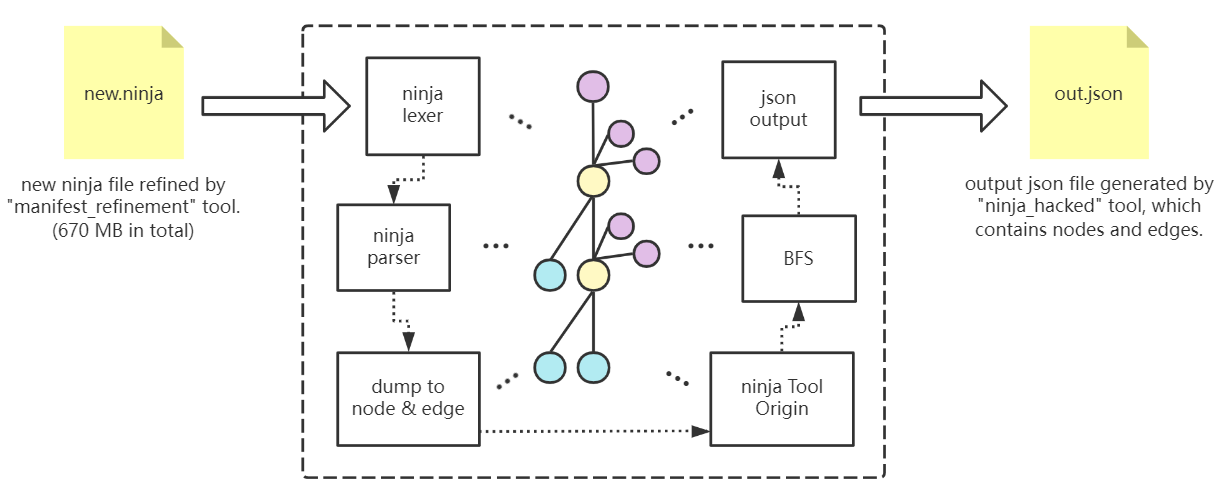
\includegraphics[width=.9\textwidth]{figures/archi-ninja-hacked.png}
    \caption{ninja\_hacked 示意图}
    \label{fig:archi-ninja-hacked}
\end{figure}

\begin{figure}[htb]
    \centering
    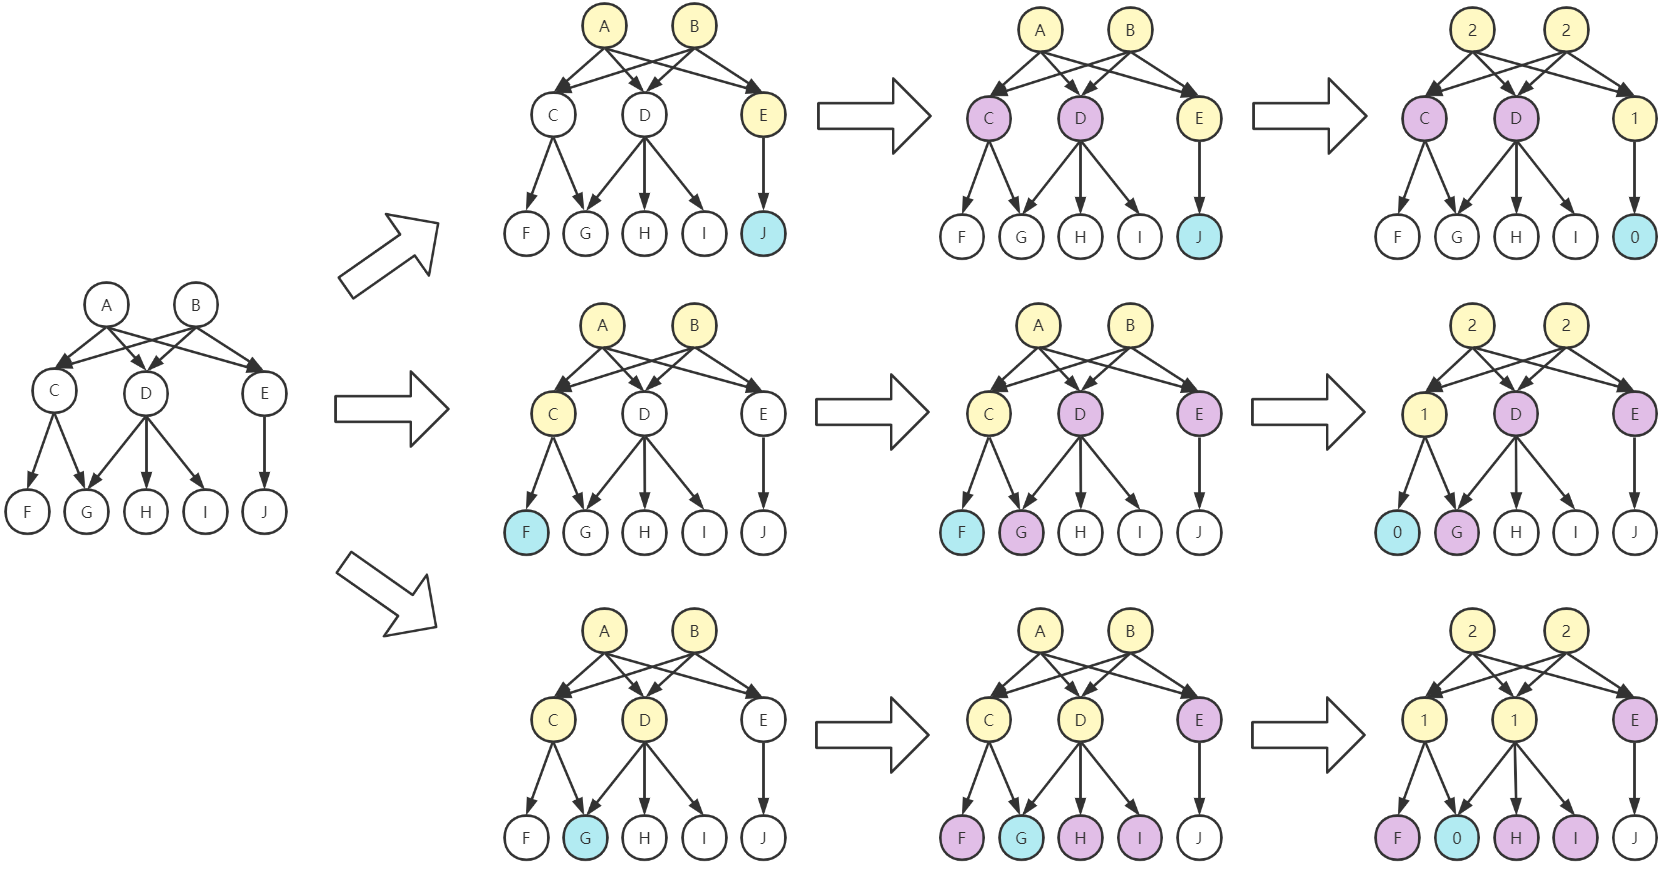
\includegraphics[width=.9\textwidth]{figures/ninja-hacked-bfs.png}
    \caption{某完全构建过程中的差异影响}
    \label{fig:ninja-hacked-bfs}
\end{figure}

\begin{figure}[htb]
    \centering
    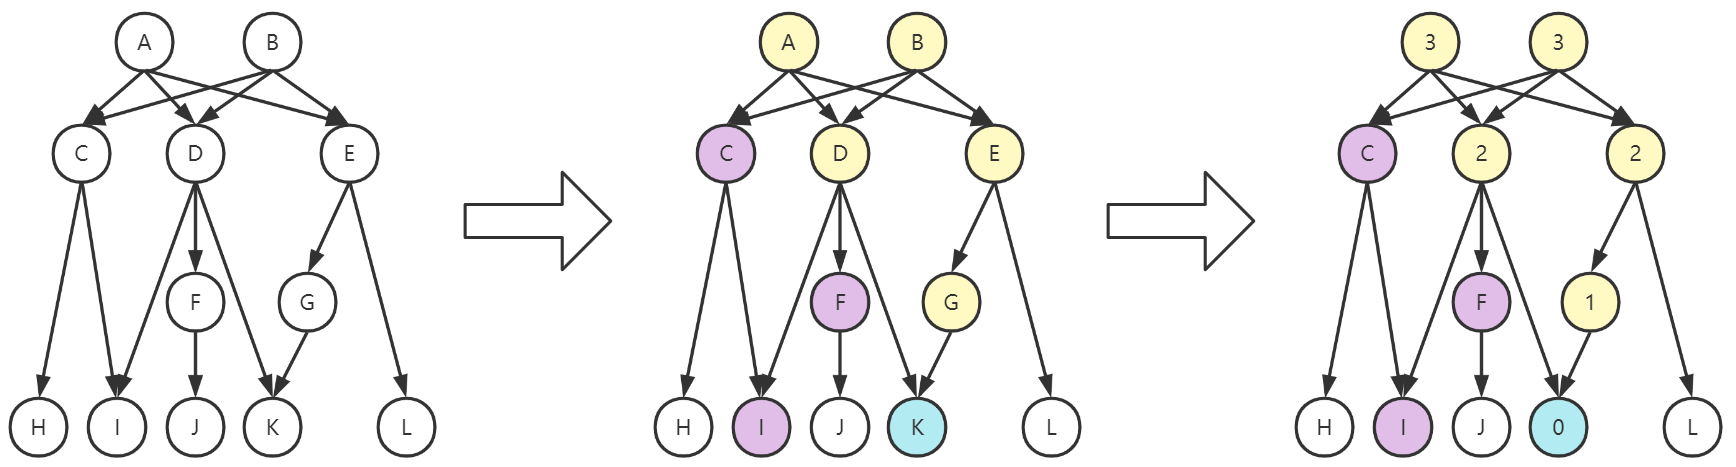
\includegraphics[width=.9\textwidth]{figures/ninja-hacked-topology-sort.png}
    \caption{使用拓扑排序思想确定完全构建过程中的距离}
    \label{fig:ninja-hacked-topology-sort}
\end{figure}

本模块需要以 Ninja 为 载体。Ninja 项目的本质是一个命令行工具,其中需要的参数都需要以命令行参数传入。Ninja 使用 ReadFlag 解析命令行参数 argv 到内部的 options 和 config 中。此后,Ninja 会进入执行构建任务的主循环中。对于主循环而言,一次循环即执行一次由一个 ninja 文件定义的完整构建过程。Ninja 中使用 ManifestParser 解析 ninja 语法,并使用其中的 Load 方法解析构建与规则,并将其全部实例化为 Edge 和 Node 对象。

Ninja\_hacked 项目巧妙借助了 Ninja 中的 “插件功能”,即 Ninja Tool。在通过命令行使用 Ninja 时,可通过指定 “-t” 参数来决定 Ninja 的行为。在 Ninja 源代码中,这些行为包括但不限于 “基于一个构建目标获得其构建过程”、“根据已部分定义的目标生成构建依赖图” 等等。ninja\_hacked 利用 Ninja 的 Tool 编写规则,集成了名为 Origin 的 Tool,该工具可以根据给定的 manifest 文件以及给定的源文件,得到其所有可能影响的源文件、中间文件与最终产物,并将这些信息以 json 形式输出到文件中。

\subsubsection{文件间影响关系可视化:deps\_reflection}

为方便展现模块间分析中文件影响关系,本系统在进行模块间分析的同时输出影响关系文件。该文件可通过 deps\_reflection 项目转化为 Graphviz 工具的输入文件。deps\_reflection 项目内部模拟了 Graphviz 内的 Node 与 Edge 数据结构,使用 ninja\_hacked 项目的输出文件作为输入,将其中的文件视作节点,将文件与文件间的依赖关系视为边,使用传统有向图构建依赖关系图。输出结果如图\ref{fig:archi-deps-reflection}所示。

\begin{figure}[htb]
    \centering
    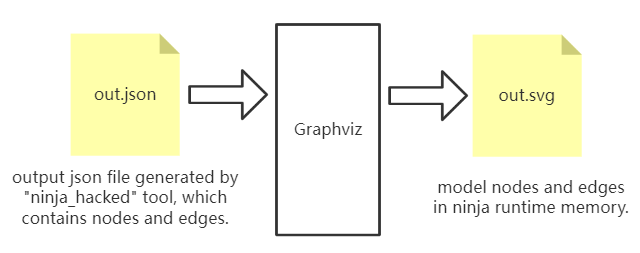
\includegraphics[width=.9\textwidth]{figures/archi-deps-reflection.png}
    \caption{deps\_reflection 示意图}
    \label{fig:archi-deps-reflection}
\end{figure}

\subsection{基于调用图的模块内分析:cg\_generator}

本系统使用调用图确定给定的变更方法对模块内其他方法造成的影响。AOSP platform/frameworks 的本质是一套有关 Android 应用开发的核心框架,用户可以通过继承等方式扩展 platform/frameworks 中定义的类。同时,platform/frameworks 中只有属于库的公共 API 的代码被库的用户扩展,所有只能通过不属于公共 API 的代码访问的代码都被认为属于库的实现。\cite{CALLGRAPHCONSTRUCTION}面向 AOSP 分析的初衷是获取两版本间软件变更对未合入主分支的代码的影响,仍旧是依托于用户应用进行的库分析,所以对库进行分析时需要关注的部分相对较少。

本系统中使用的调用图生成装置基于开源工具 Java Call Graph 开发,增加了对 AOSP 中构建产物的适配,完善了以方法调用指令为基础的访问者模式,可以根据变更方法的类名与方法名获取其影响的方法集合。该部分架构如图\ref{fig:archi-cg-generator}所示,调用图生成部分的函数逻辑如图\ref{fig:cg-generator-jcallgraph}所示。

\begin{figure}
    \centering
    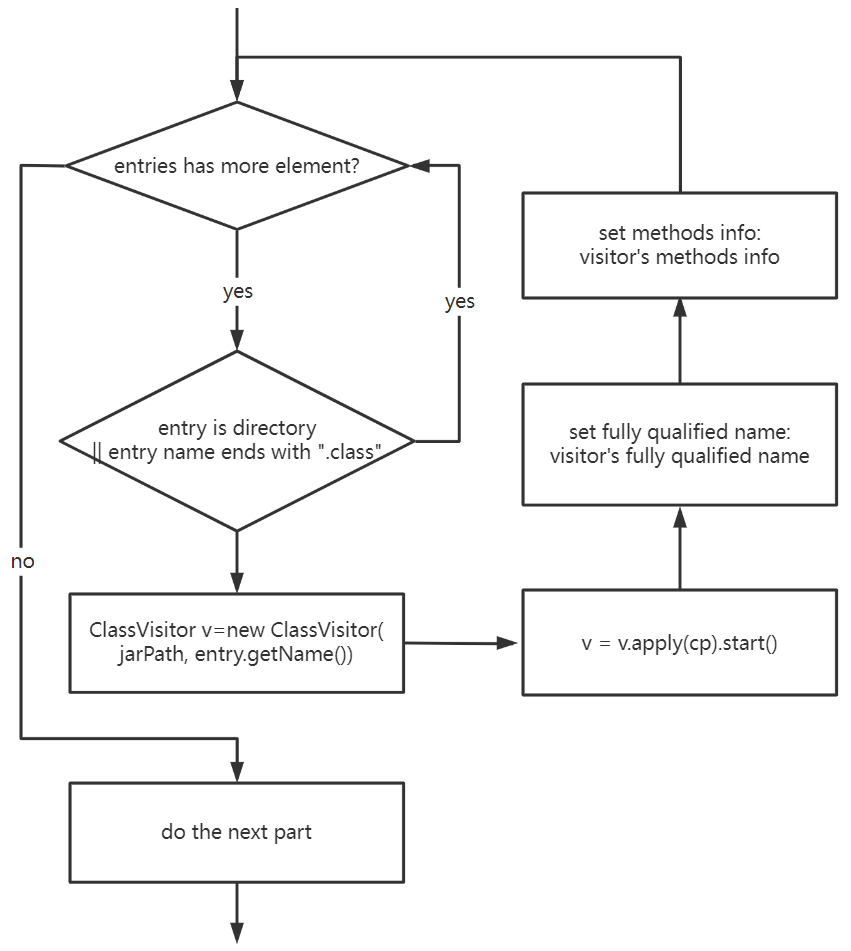
\includegraphics[width=.9\textwidth]{figures/cg-generator-jcallgraph.png}
    \caption{cg\_generator 调用图生成部分的函数逻辑}
    \label{fig:cg-generator-jcallgraph}
\end{figure}

cg\_generator 模块需要传入真实存在的 jar 文件。在具体实现上,项目使用 util.jar 中的 JarFile 与 JarInfo 获得 jar 文件内各 class 文件入口以及 jar 文件元信息。对于每一个 class 文件,项目都使用一个独立的 Apache BCEL 中的 ClassParser 解析字节码获得 JavaClass 类的实例化对象。针对每一个 JavaClass,项目中使用自定义的具体访问者 ClassVisitor 进行独立分析。JavaClass 中存在本属于字节码文件内但已被解析的常量池、属性表集合以及方法表集合等概念。方法表集合中存放了访问标志与各类索引\cite{UNDERSTANDINGJVM}。对于 JavaClass 对象内的每个方法,ClassParser 已将其实例化为一系列 Method 对象。在方法属性表中的 Code 属性里,存放了方法的字节码指令集合\cite{UNDERSTANDINGJVM}。针对每一个 Method,项目中又使用自定义的具体访问者 MethodVisitor 进行独立分析。每个 Method 中都存在一条由一系列类型不同但都继承于同一父类 Instruction 的子类组成的链表,因此 MethodVisitor 遍历当前方法下的所有 instruction,对每条 instruction 都进行判断,确定在生成方法调用图这一场景下是否需要将其纳入考虑范围内。诸如上述中 JavaCLass、Method、Instruction 等在内存中不可修改的数据结构,以 Instruction 类为例,Apache BCEL 使用如图\ref{fig:cg-generator-object-structure}所示的关系提供用户可自定义新操作方法的接口。

\begin{figure}[htb]
    \centering
    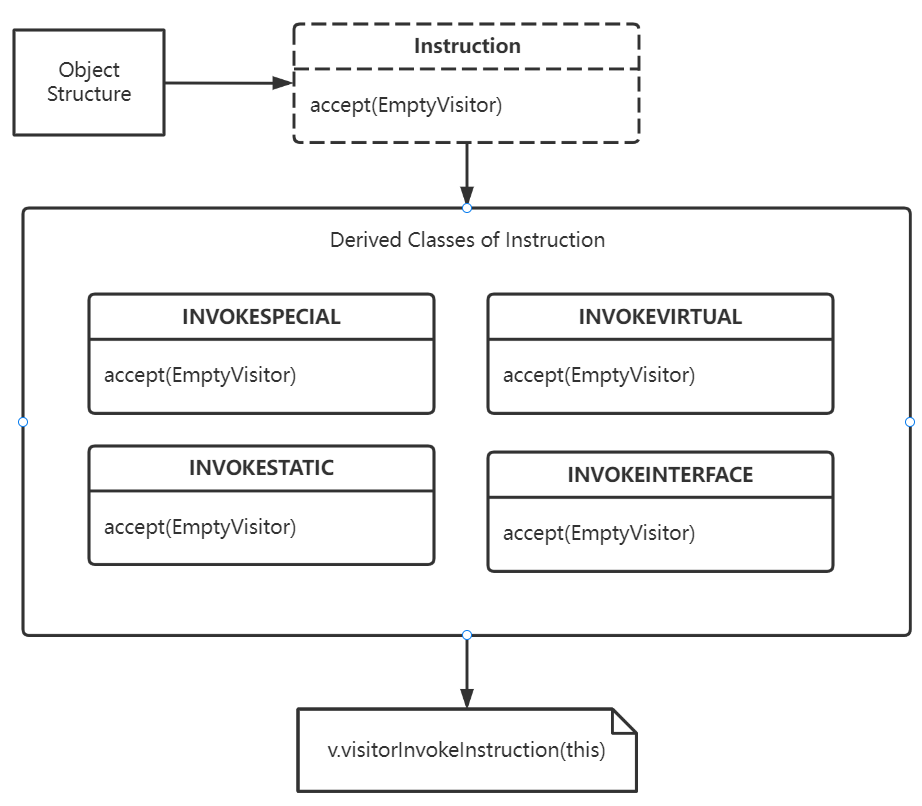
\includegraphics[width=.8\textwidth]{figures/cg-generator-object-structure.png}
    \caption{Instruction 基类、派生类与具体元素之间的关系}
    \label{fig:cg-generator-object-structure}
\end{figure}

对于 Java 语言,Java 7 增加的 invokedynamic 指令是使用字节码文件分析调用图的问题之一,并且在 Java 8 中新增的 Lambda 函数底层便是使用该 JVM 指令执行。invokedynamic 指令原本有 4 个操作数,其中前两个操作数共同构成了查找常量池中 CONSTANT\_InvokeDynamic\_info 的索引,以便于查找 Bootstrap method 并将参数传入。对于每一条 invokedynamic 指令执行的位置,JVM 都将其视为一个动态调用点,cg\_generator 模块使用容器来存储调用点所在的方法以及调用的目标。

为使用 Apache BCEL 提供的访问者模式接口,需要定义一系列访问者。由于本系统构建调用图不需要与方法同级别的信息(如函数形参类型、返回值类型等),所以在 cg\_generator 中,总共定义了 ClassVisitor 与 InstructionVisitor 两类具体访问者以及作为假访问者的 MethodVisitor。访问者与具体访问者间的关系如图\ref{fig:cg-generator-client}所示。需要说明的是,由于 JavaClass 中成员与 Method 中成员大致相仿(JavaClass 下有 Method 列表,Method 下有 Instruction 链表),纵使 MethodVisitor 并未覆写任何访问者模式相关的方法,但 ClassVisitor 与 MethodVisitor 的设计仍然十分相似。

\begin{figure}[htb]
    \centering
    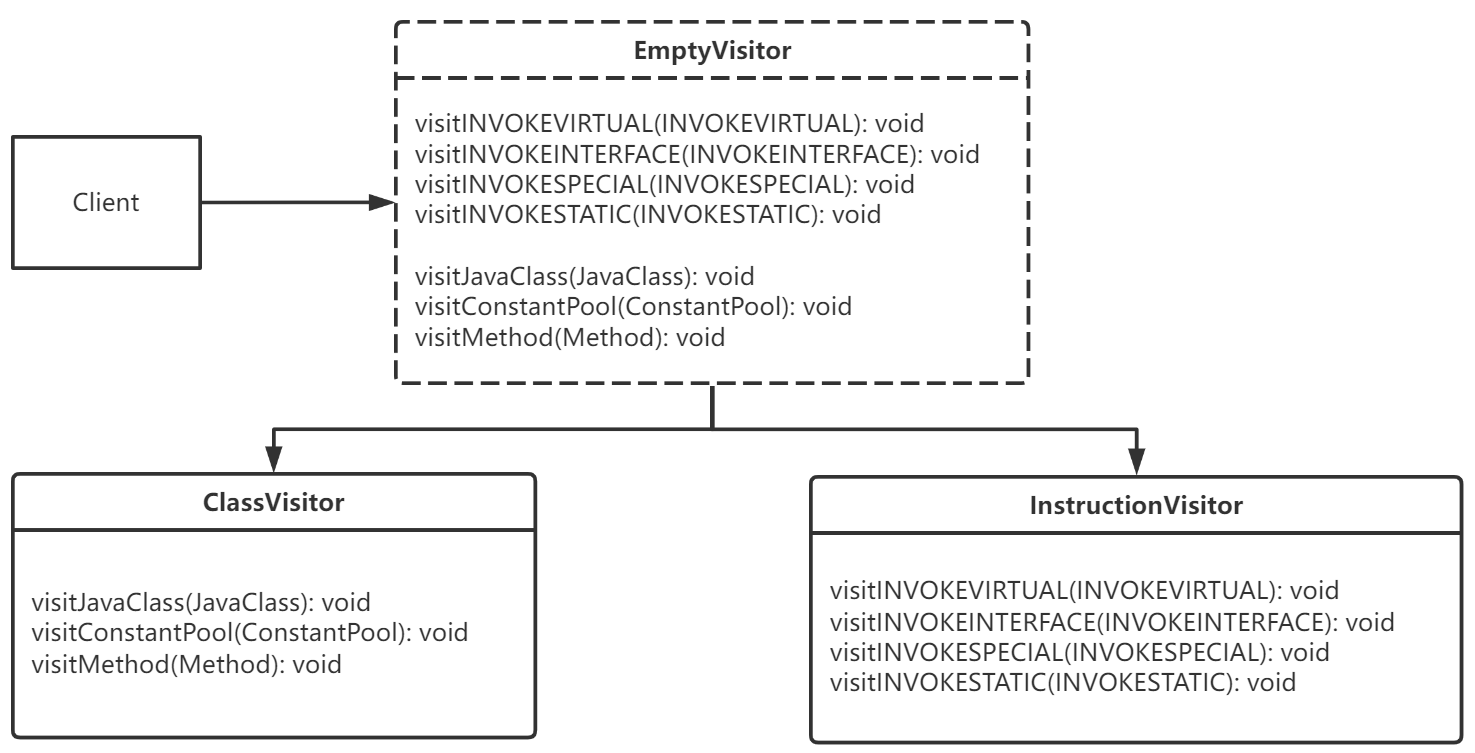
\includegraphics[width=.9\textwidth]{figures/cg-generator-client.png}
    \caption{访问者 EmptyVisitor 与具体访问者 ClassVisitor / InstructionVisitor 之间的关系}
    \label{fig:cg-generator-client}
\end{figure}

\begin{figure}[htb]
    \centering
    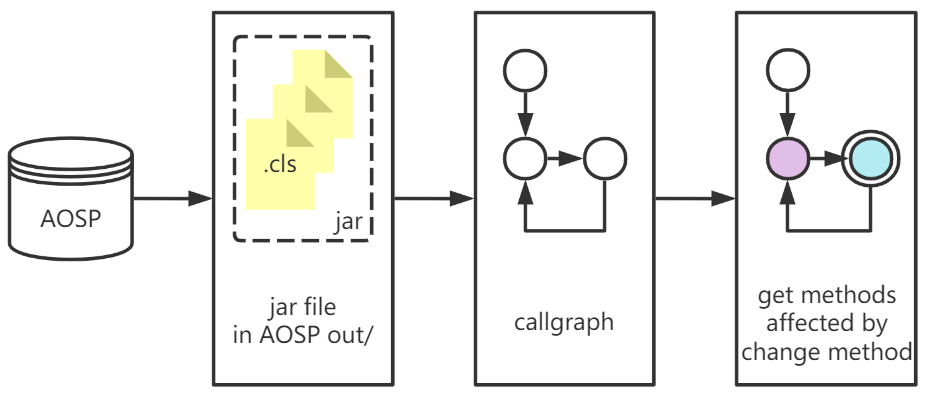
\includegraphics[width=.9\textwidth]{figures/archi-cg-generator.png}
    \caption{cg\_generator 示意图}
    \label{fig:archi-cg-generator}
\end{figure}

\subsection{模块实验结果}

\subsubsection{Repo\_crawler 实验结果}

AOSP 中仓库分布并无规则,存在两同级目录属于不同仓库的情况(如 platfrom/frameworks/av 与 platform/frameworks/native),但同时也存在多级目录作为仓库被维护的情况(如 platform/frameworks/opt/bitmap 与 platform/frameworks/opt/car/services)。因此需要即时爬取并解析 googlesource 上的数据。 该系统利用 Python 的 requests 和 bs4 获取 platform/frameworks 下的 67 个仓库名称。该小型应用工具作为模块间分析流程的第一步,模块设计如图\ref{fig:design-repo-list}所示,具体实现可见 \href{https://github.com/AOSPworking/repo_crawler}{repo\_crawler}。

\begin{figure}[htb]
    \centering
    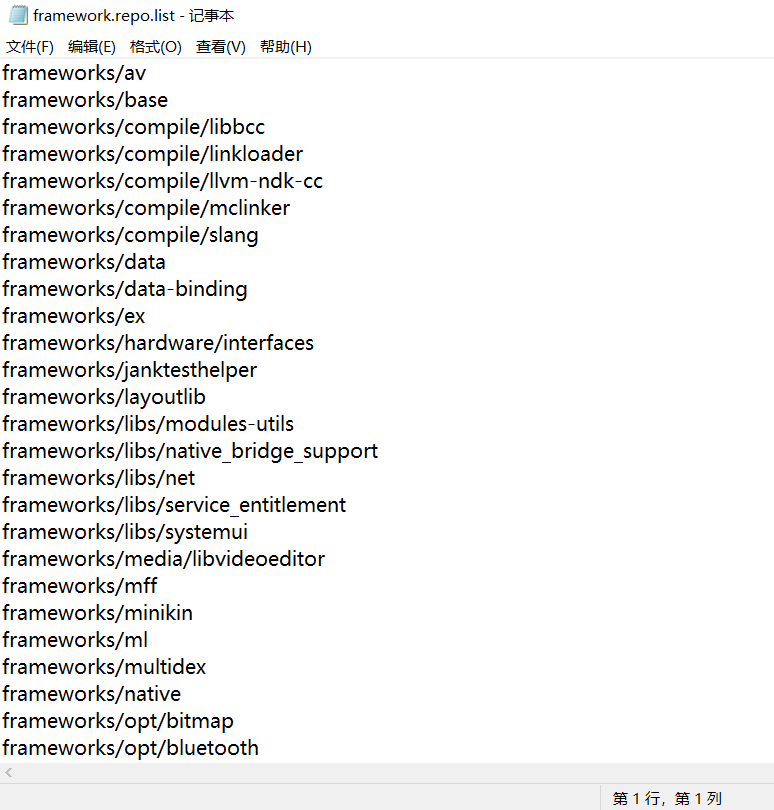
\includegraphics[width=.4\textwidth]{figures/design-repo-list.png}
    \caption{爬取 frameworks 下所属仓库获得的名称列表}
    \label{fig:design-repo-list}
\end{figure}

\subsubsection{Pkg\_repo\_tool 实验结果}

仿照 soong 构建系统在运行初调用 Blueprint 模块的行为。bp\_collector 旨在获取给定路径下的所有 Android.bp 文件。bp\_collector 选择借助 soong 构建系统运行时输出的 Android.bp.list 文件,该文件是 soong 运行时收集各路径下 Android.bp 文件的依据,存储在 out/.module\_paths 下。bp\_collector 正是依靠该文件的生成逻辑,从 AOSP 中各目录中获取文件,并存储在指定的文件夹下,以方便后续分析。

由于 AOSP 下的 Blueprint 项目是一个较为独立的项目,相较于 soong 这一必须基于 AOSP 目录结构才能运行的系统,Blueprint 更像是为 soong 提供有关 bp 文件操作能力的插件。根据 bp\_collector 的执行结果,pkg\_repo\_tool 模块内部利用 Blueprint 中的 parser 模块解析收集到的 bp 文件,获得仓库到模块的关系如图\ref{fig:design-repo-pkg-relation}所示,该模块具体实现可见 \href{https://github.com/AOSPworking/pkg_repo_tool}{pkg\_repo\_tool}。

\begin{figure}[htb]
    \centering
    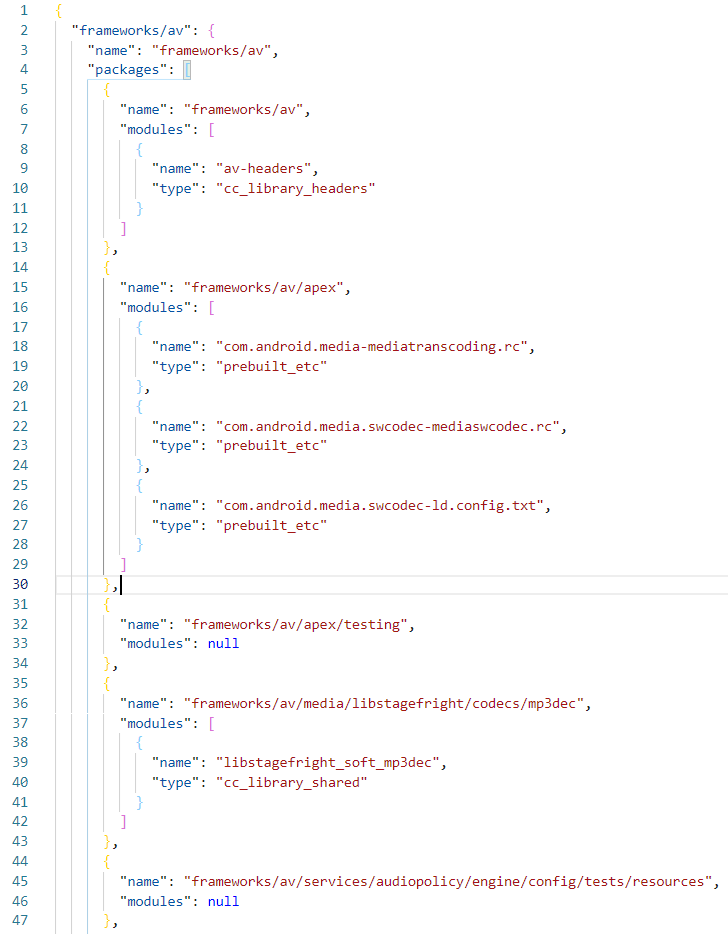
\includegraphics[width=.4\textwidth]{figures/design-repo-pkg-relation.png}
    \caption{解析得到 AOSP 下各仓库内模块情况}
    \label{fig:design-repo-pkg-relation}
\end{figure}

\subsubsection{Diff\_extractor 实验结果}

通过输入给定仓库所在路径与两个版本的 commit id,借助 .git 目录下 的数据结构,获得通过 jgit 库效仿 git diff 指令获得两版本间差异(在 jgit 中,用于描述差异的类被称作 DiffEntry,通过 DiffEntry 可以获得存在差异的文件名以及具体文本差异)。本系统选用 GumTree 作为抽象语法树节点级别的变更获取工具。通过 DiffEntry 中获得的文件名以及输入的 commit id,可从 .git 中的对象文件中获取对应 commit id 下指定路径文件内容。使用算法\ref{alg:get-method-name},可从 GumTree 给出的变更节点向上回溯至方法定义节点与类定义节点。结果如图\ref{fig:design-diff-extractor}所示,该模块具体实现可见 \href{https://github.com/AOSPworking/diff_extractor}{diff\_extractor}。

\begin{figure}[htb]
    \centering
    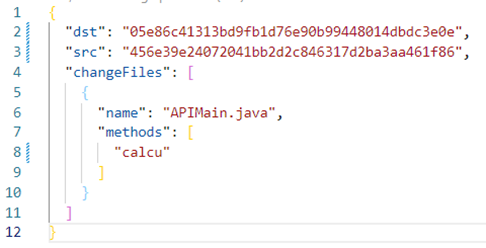
\includegraphics[width=.4\textwidth]{figures/design-diff-extract.png}
    \caption{扫描 AOSP 编译产物获得存在变更的类以及方法的元数据信息}
    \label{fig:design-diff-extractor}
\end{figure}

\subsubsection{Manifest\_refinement 实验结果}

用于描述 AOSP 完全构建过程的纯文本文件 build.ninja 仍需要占用 3 GB 左右的磁盘空间,在使用 manifest\_refinement 项目对 build.ninja 文件按条件过滤后,得到的 new-build.ninja 仅有 670 MB 左右。由于扩展有向图的复杂程度与 $O(F + B)$ 有关,而 build.ninja 中的文件中大多数篇幅在定义扩展有向边,因此对 build.ninja 文件的精简可以有效缩减对 ninja\_hacked 项目进行分析时需要的资源。manifest 文件处理结果如图\ref{fig:archi-manifest-refinement}所示,该模块具体实现可见 \href{https://github.com/AOSPworking/manifest_refinement}{manifest\_refinement}。

\begin{figure}[htb]
    \centering
    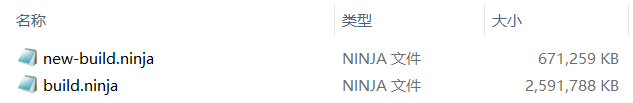
\includegraphics[width=.9\textwidth]{figures/design-manifest.png}
    \caption{AOSP 构建过程描述文件 build.ninja 处理结果}
    \label{fig:design-manifest}
\end{figure}

\subsubsection{Ninja\_hacked 实验结果}

相较于插桩、获取运行时内存的手段,借助 Ninja 中的 Node 与 Edge,充分重用已有数据结构编写程序,并将其集成到原有项目中的方法更加具有操作性。Ninja 中使用 Node 抽象真实存在的文件,使用 Edge 抽象单一构建过程,利用 diff\_extractor 模块的输出作为本模块的输入,获得两版本间存在代码变更的文件名。在 Ninja 所维护的有向无环图中,源代码文件对应的 Node 仅有 in\_edge,而其 out\_edge 不存在或 out\_edge 并没有连接其余输出。进而可以使用广度优先搜索算法,得到的因变动而被影响的文件列表,结果如图\ref{fig:design-node}所示。

在此基础上,运用算法\ref{alg:intermodule-analysis}可以得到 AOSP 构建中所有因给定变更文件集合而受到直接或间接影响的文件集合。描述此类影响关系的内容如图\ref{fig:design-edge}所示。该模块具体实现可见 \href{https://github.com/AOSPworking/ninja-hacked}{ninja\_hacked}。

\begin{figure}[htb]
    \centering
    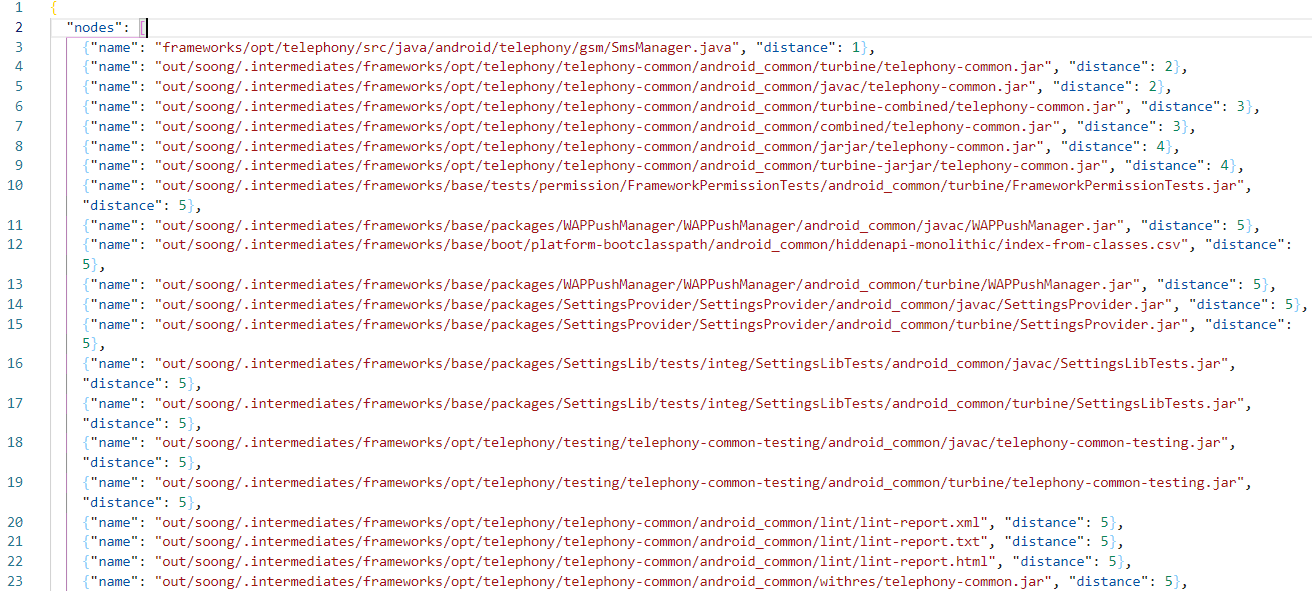
\includegraphics[width=.9\textwidth]{figures/design-node.png}
    \caption{基于给定变更而遭到影响的文件列表}
    \label{fig:design-node}
\end{figure}

\begin{figure}[htb]
    \centering
    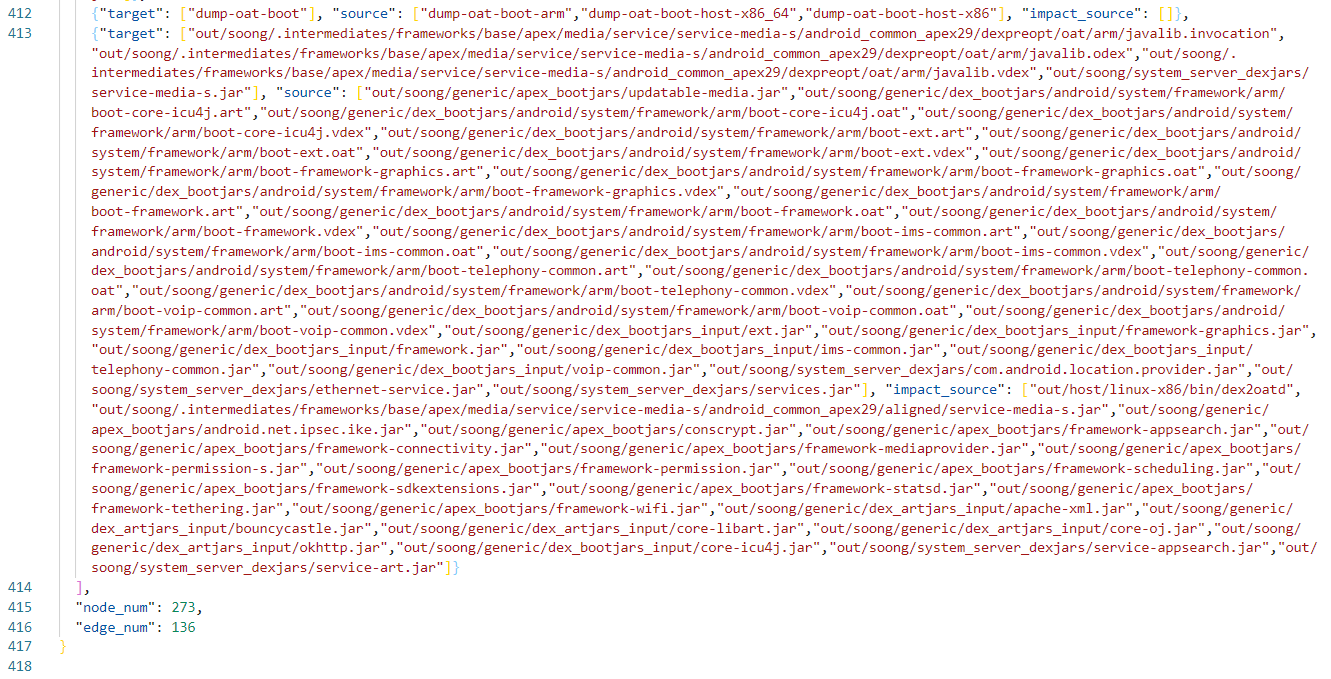
\includegraphics[width=.9\textwidth]{figures/design-edge.png}
    \caption{ninja\_hacked 输出文件中描述的文件间影响关系}
    \label{fig:design-edge}
\end{figure}

\subsubsection{Deps\_reflection 实验结果}

deps\_reflection 使用 Graphviz 展现模块间分析中文件影响关系。本模块使用了 ninja\_hacked 模块输出的 json 文件,使用 JavaScript Graphviz 库中定义的 node 与 edge 类模拟 json 中定义的对象,使用传统的有向图构建依赖关系图。由于 AOSP 体积过于庞大,构建过程过于复杂,以至于一个源文件能够直接影响的中间产物与目标产物以及构建过程就有上百个。因此为可视化更为美观,deps\_reflection 屏蔽了间接影响的文件。由于本模块仅仅用于可视化,并不修改 ninja\_hacked 的输出文件,因此屏蔽间接影响文件是可行的。该模块输出结果如图\ref{fig:design-deps-reflection}所示,具体实现可见 \href{https://github.com/AOSPworking/deps_reflection}{deps\_reflection}。

\begin{figure}[htb]
    \centering
    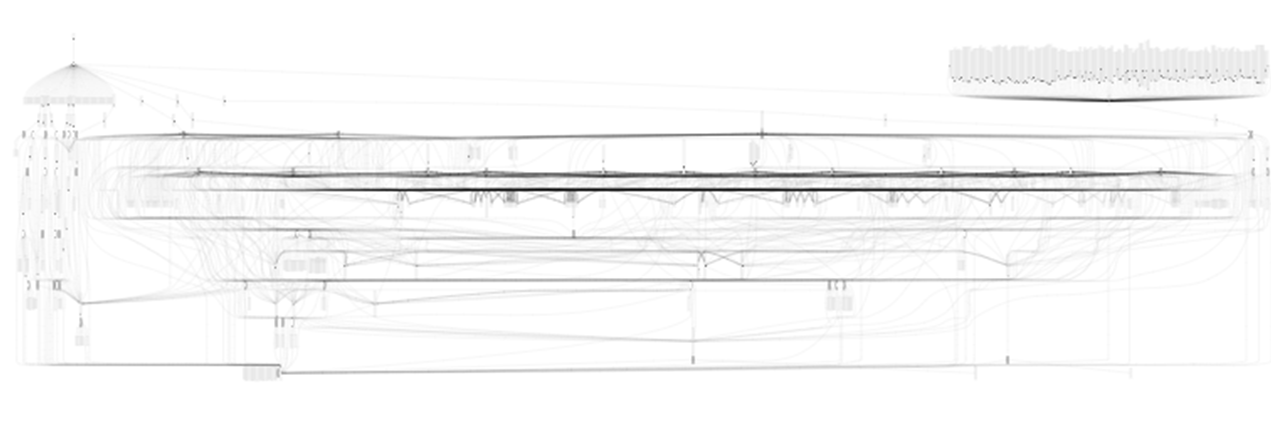
\includegraphics[width=.9\textwidth]{figures/design-view.png}
    \caption{deps\_reflection 构建的依赖关系图}
    \label{fig:design-deps-reflection}
\end{figure}

\begin{figure}[htb]
    \centering
    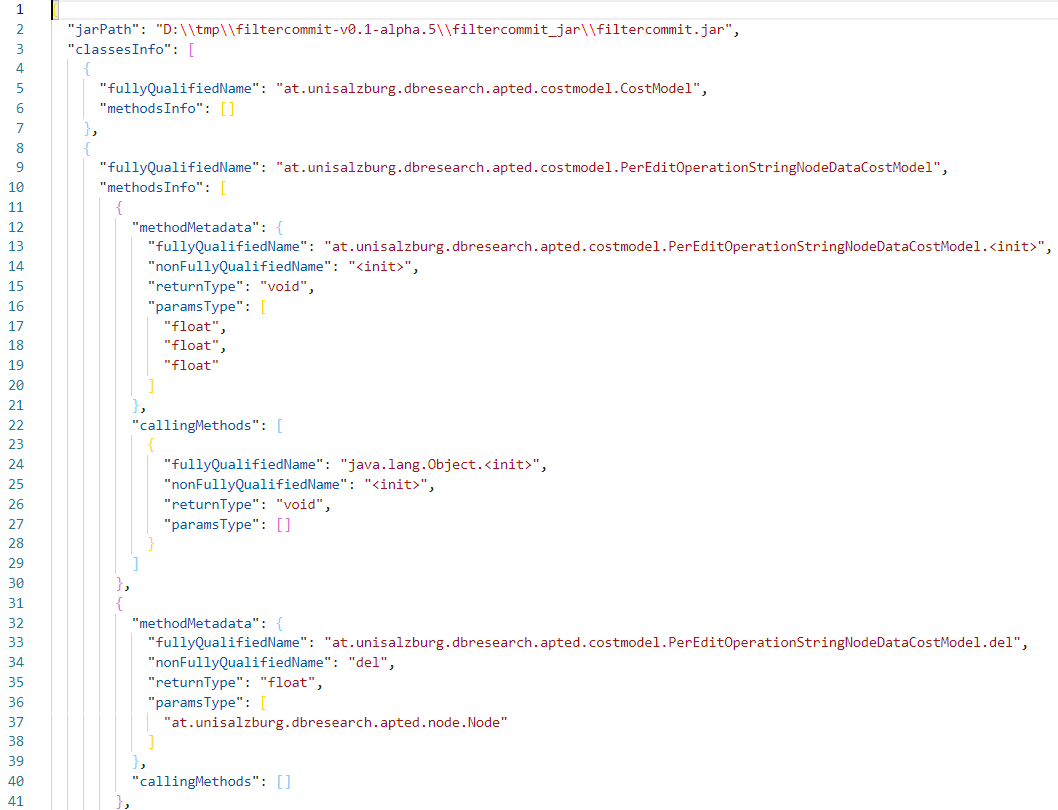
\includegraphics[width=.6\textwidth]{figures/design-cg-generator.png}
    \caption{方法调用图中保存的元数据信息}
    \label{fig:design-cg-generator}
\end{figure}

\subsubsection{Cg\_generator 实验结果}

cg\_generator 中所使用的调用图构建方法基于 Java Call Graph 开发。Java Call Graph 使用访问者模式这一时常出现在各类静态程序分析框架中的设计模式开发。访问者模式着重于对某个对象中各个元素的操作的自定义,访问者模式适用于无法接触被操作类源代码的场景,开发者通过该模式可以增加面向对象内各层级元素的新操作方法\cite{gamma1994design}。

我在原本的 Java Call Graph 基础上,拆分了并部分重写了针对 method 与 instruction 两种类的访问方式,我所作出的改进大幅度改善了项目代码的可读性和可扩展性,可以针对 method 与 instruction 明确地进行不同的分析。具体而言,项目使用了 Apache BCEL 字节码操作库,确定给定的变更方法以及方法内的方法调用状况。在为所涉及的方法创建节点(包括实际节点与虚拟节点)的同时,构建方法与方法间的调用关系图,即对模块内其他方法造成的影响。完善的以方法调用指令为基础的访问者模式,可以根据变更方法的类名与方法名获取其影响的方法集合。除此之外,我增加了对 AOSP 结构与其中构建产物的适配(如 AOSP 构建过程得到的 jar 包中的部分 class 文件可能存在无代码区的问题)。所得结果如图\ref{fig:design-cg-generator}所示,该模块具体实现可见 \href{https://github.com/AOSPworking/cg_generator}{cg\_generator}。

综上所述,本文所设计的软件变更分析系统在 AOSP 场景下重点体现在 “依照构建系统完成数据处理”、“变更获取”、“模块间分析” 以及 “模块内分析” 三点。本系统以 AOSP 下的 platform/frameworks 为例,在数据预处理方面获得其下的 67 个仓库,并与 5804 个模块建立了联系;在变更获取方面,根据给定的仓库路径和 commit id,能够成功做到获取存在变更的方法以及所属类;在模块间分析方面,成功将 2.7GB 的 build.ninja 文件精简为 670MB,大幅缩小了分析范围,且能够根据给定源文件使用 Ninja 内部数据结构导出全部影响关系;在模块内分析方面,能够根据给定的 jar 文件得到调用图,并根据输入的方法名得到所有与该方法相关的方法列表。
